%%%%%%%%%%%%%%%%%%%%%%%%%%%%%%%%%%%%%%%%%
% Programming/Coding Assignment
% LaTeX Template
%
% This template has been downloaded from:
% http://www.latextemplates.com
%
% Original author:
% Ted Pavlic (http://www.tedpavlic.com)
%
% Note:
% The \lipsum[#] commands throughout this template generate dummy text
% to fill the template out. These commands should all be removed when 
% writing assignment content.
%
% This template uses a Perl script as an example snippet of code, most other
% languages are also usable. Configure them in the "CODE INCLUSION 
% CONFIGURATION" section.
%
%%%%%%%%%%%%%%%%%%%%%%%%%%%%%%%%%%%%%%%%%

%----------------------------------------------------------------------------------------
%	PACKAGES AND OTHER DOCUMENT CONFIGURATIONS
%----------------------------------------------------------------------------------------

\documentclass{article}

\usepackage{fancyhdr} % Required for custom headers
\usepackage{lastpage} % Required to determine the last page for the footer
\usepackage{extramarks} % Required for headers and footers
\usepackage[usenames,dvipsnames]{color} % Required for custom colors
\usepackage{graphicx} % Required to insert images
\usepackage{listings} % Required for insertion of code
\usepackage{courier} % Required for the courier font
\usepackage{multirow}
\usepackage{hyperref}


% Margins
\topmargin=-0.45in
\evensidemargin=0in
\oddsidemargin=0in
\textwidth=6.5in
\textheight=9.0in
\headsep=0.25in

\linespread{1.1} % Line spacing

%----------------------------------------------------------------------------------------
%	CODE INCLUSION CONFIGURATION
%----------------------------------------------------------------------------------------

\definecolor{MyDarkGreen}{rgb}{0.0,0.4,0.0} % This is the color used for comments
\lstloadlanguages{c} % Load Perl syntax for listings, for a list of other languages supported see: ftp://ftp.tex.ac.uk/tex-archive/macros/latex/contrib/listings/listings.pdf
\lstset{language=[sharp]c, % Use Perl in this example
        frame=single, % Single frame around code
        basicstyle=\small\ttfamily, % Use small true type font
        keywordstyle=[1]\color{Blue}\bf, % Perl functions bold and blue
        keywordstyle=[2]\color{Purple}, % Perl function arguments purple
        keywordstyle=[3]\color{Blue}\underbar, % Custom functions underlined and blue
        identifierstyle=, % Nothing special about identifiers                                         
        commentstyle=\usefont{T1}{pcr}{m}{sl}\color{MyDarkGreen}\small, % Comments small dark green courier font
        stringstyle=\color{Purple}, % Strings are purple
        showstringspaces=false, % Don't put marks in string spaces
        tabsize=5, % 5 spaces per tab
        %
        % Put standard Perl functions not included in the default language here
        morekeywords={rand},
        %
        % Put Perl function parameters here
        morekeywords=[2]{on, off, interp},
        %
        % Put user defined functions here
        morekeywords=[3]{test},
       	%
        morecomment=[l][\color{Blue}]{...}, % Line continuation (...) like blue comment
        numbers=left, % Line numbers on left
        firstnumber=1, % Line numbers start with line 1
        numberstyle=\tiny\color{Blue}, % Line numbers are blue and small
        stepnumber=5 % Line numbers go in steps of 5
}

\newcommand{\horrule}[1]{\rule{\linewidth}{#1}}

\newcommand\doubleplus{\ensuremath{\mathbin{+\mkern-10mu+}}}

% Creates a new command to include a perl script, the first parameter is the filename of the script (without .pl), the second parameter is the caption
\newcommand{\perlscript}[2]{
\begin{itemize}
\item[]\lstinputlisting[caption=#2,label=#1]{#1.cs}
\end{itemize}
}

\begin{document}

\begin{tabular}{l l}
\multirow{5}{*}{
\includegraphics[width=2cm]{../../recursos/logo.png}} & Universidad del Istmo de Guatemala \\
 & Facultad de Ingenieria \\
 & Ing. en Sistemas \\
 & Informatica II \\
 & Prof. Ernesto Rodriguez - \href{mailto:erodriguez@unis.edu.gt}{erodriguez@unis.edu.gt} \\
\end{tabular}
\\\\\\

\begin{center}
        \horrule{0.5pt}
        \huge{Laboratorio \#3} \\
        \large{Fecha de entrega: 14 de Febrero, 2019 - 11:59pm} \\
        \horrule{1pt}
\end{center}

\emph{Instrucciones: Resolver cada uno de los ejercicios siguiendo sus respectivas
instrucciones. El trabajo debe ser entregado a traves de Github, en su repositorio del curso, colocado en una carpeta llamada "Laboratorio \#3".
Al menos que la pregunta indique diferente, todas las respuestas a preguntas escritas deben presentarse en
un documento formato pdf, el cual haya sido generado mediante Latex. Este laboratorio
debe ser elaborado en parejas.}

\section*{Tarea \#1 (70\%)}

A continuaci\'on se presenta un \emph{diagrama de flujo}. Implemente utilizando C++ un programa
que opere segun especifica dicho diagrama. La siguiente tabla le especificara el caracter, gravedad
y resistencia de viento para cada uno de los cuerpos celestes que debe trabajar su programa:
\\\\
\begin{tabular}{|c|c|c|c|}
    \hline
    {\bf Cuerpo} & {\bf Caracter} & {\bf Gravedad} & {\bf Resistencia} \\
    \hline
    Tierra & t & 9.8 & 0.0023 \\
    \hline
    Venus & v & 8.87 & 0.0023 \\
    \hline
    Luna & l & 1.62 & 0 \\
    \hline
    Callisto & c & 1.23 & 0 \\
    \hline
\end{tabular}
Puede suponer que el objeto en caida libre tiene 1 kilogramo de masa y su area es de 1 metro cuadrado, por lo cual:
\begin{enumerate}
    \item{$F_{atm}=kv^2$}
    \item{$F=g-F_{atm}$}
    \item{$a=F$}
    \item{$v=at$}
    \item{$d=vt$}
\end{enumerate}
Donde:
\begin{enumerate}
    \item{$F_{atm}$ es la fuerza debido a la resistencia del viento}
    \item{$k$ es la constante de resistencia del viento}
    \item{$t$ es el tiempo}
    \item{$v$ es la velocidad}
    \item{$a$ es la aceleraci\'on}
    \item{$g$ es la fuerza ejercida por la gravedad del cuerpo celeste.}
\end{enumerate}

Para esta tarea, a diferencia del {\bf ejemplo en clase}, debe utilizar intervalos de duraci\'on de
$0.01s$ para hacer sus calculos (no de $1s$).

\begin{center}
    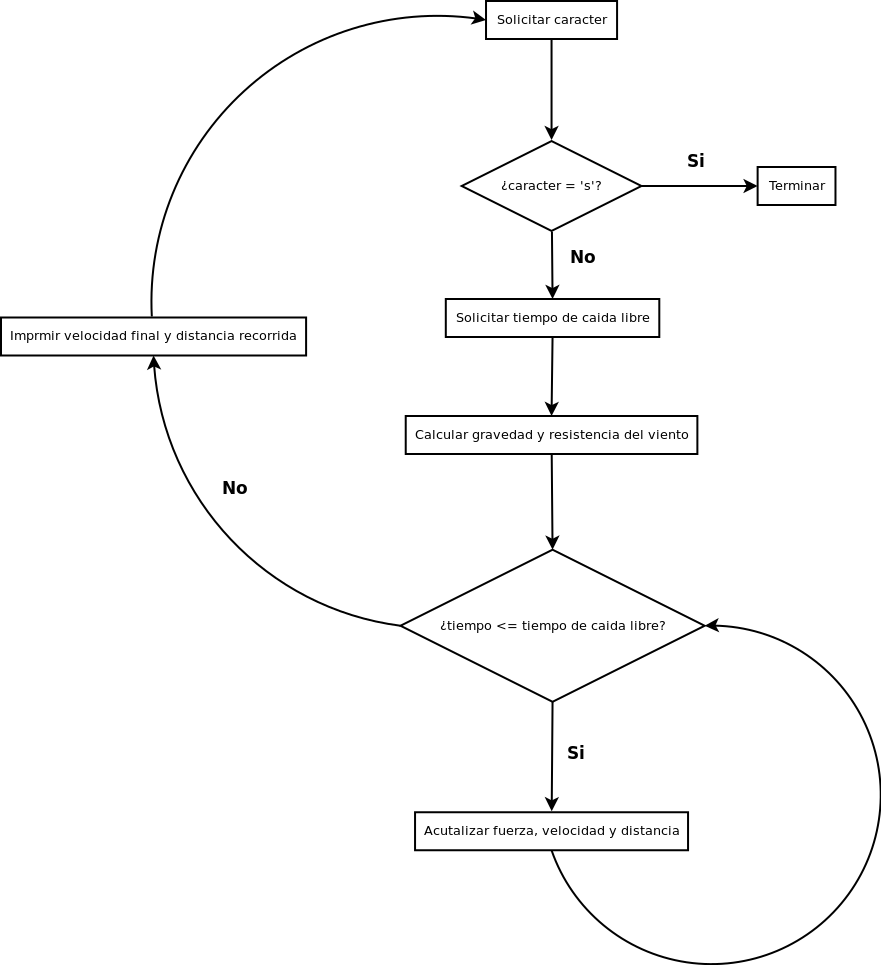
\includegraphics[width=12cm]{Flujo.png}
\end{center}

\section*{Tarea \#2 (30\%)}
El programa anterior no especifica que hacer cuando se ingresa un caracter desconocido, como por ejemplo
el caractar 'x'. Su tarea es:
\begin{enumerate}
    \item{Divisar una estrategia para manejar estos casos extraordinarios}
    \item{Extienda el diagrama de flujo adjunto en esta carpeta. Puede utilizar el programa
    Dia (\url{http://dia-installer.de/}) para actualizar el diagrama.}
    \item{Implemente su estrategia en el programa que sera entregado.}
\end{enumerate}
\end{document}